\documentclass[11pt]{article}

\usepackage{float}
\usepackage{hyperref}
\usepackage{fullpage}
\usepackage{verbatim}
\usepackage{moreverb}
\usepackage{graphicx}
\usepackage{minted}
\let\verbatiminput=\verbatimtabinput
\def\verbatimtabsize{4\relax}

\begin{document}
\title{EECS 151/251A FPGA Lab\\
Lab 4: Rotary Encoder and debouncer, Testbench tools, Sequencer}

\author{Prof. Borivoje Nikolic \\
TA: Vighnesh Iyer \\Department of Electrical Engineering and Computer Sciences\\
College of Engineering, University of California, Berkeley}
\date{}
\maketitle

\section{Before You Start This Lab}

Before you proceed with the contents of this lab, we suggest that you review the three documents from last lab.

\begin{enumerate}
	\item \textbf{labs\_fa16/docs/Verilog/verilog\_fsm.pdf} - Goes over concepts of FSM in Verilog. Provides an example of  implementing FSM's in Verilog and pitfalls to watch out for.
	
	\item \url{http://www.labbookpages.co.uk/electronics/debounce.html} - Read "What is Switch Bounce" section to get idea of why we need a debouncer circuit. Read the "Digital Switch Debouncing" section to get a general overview of the circuit, its parts, and their purpose. You may want to pay attention to the purpose of the synchronizer as meta-stability is something you will go over in class. 
	
	\item \url{http://www.xilinx.com/products/boards/s3estarter/files/s3esk_rotary_encoder_interface.pdf} - Read page 5 (Rotary Encoder and Signals) to get an idea of how the encoder works and the signal it generates. You can read the next few pages to get a better idea of how to use the signals. 

\end{enumerate}

For the first part of the lab, we will fix an issue most rotary encoders had using a debouncer circuit and elaborate on the changes you have to make to the debouncer circuit between the buttons and rotary encoder. We will give you some testbenches for these circuits and introduce you to some tools Verilog provides for making debugging easier. Finally, you will use what you've made so far to create a sequencer where you will use synchronous RAM as memory to store your tune.

\subsection{Helpful Hint: Synthesis Warnings and Errors}
At various times in this lab, things will just not work on the FPGA or in simulation. To help with debugging, you can run \verb|make synth| in the \verb|lab2/| folder. This will just run \verb|xst| which will only take a few seconds. Then you should run \verb|make report|. In the window that opened, click on \verb|Synthesis Messages| on the left under \verb|Errors and Warnings|. Any synthesis warnings you see here are a possible alert to some issue in your circuit. If you don't understand a warning, ask a TA; it almost always reveals some issue in your RTL.

If your reports indicate there are no issues but you still have problems, please make sure that it is working in simulation. There is one case related to how memory is generated where you will likely get different results between simulation and actual FPGA behavior but we do not expect it to occur in this lab. 
 
\section{Lab Overview}

In this lab, we will begin by taking your rotary encoder circuit and adding a debouncer in front it. With the implementation from last lab, some rotary encoders would interpret more rotations than expected. We will add a debouncer to get reduce glitched or buggy signals

\section{Debouncer Review}
Last lab, there were some questions about using an array for the debouncer. We will elaborate more and review the debouncer circuit so there is less confusion this time. 

The debouncer for one button uses two counters. Let us start with the saturating counter. The saturating counter receives two essential signals: the synchronized input and an enable signal. Every time the enable signal goes high, one of the two things can happen:

- if the input synchronized signal was high, we increment the counter. Once this counter equals \verb|PULSE_COUNT_MAX|, we indicate the button has been pressed long enough. The larger \verb|PULSE_COUNT_MAX| is, the longer we have to hold the button for the circuit to realized we actually pushed the button.
- if the input synchronized signal was low, we reset the counter. This essentially means we stopped pressing the button before the circuit realized we pushed the button.

The wrapping counter essentially tells the saturating counter when to count. Everything we reach \verb|SAMPLE_COUNT_MAX|, we tell the saturating counter to count by one For example, if we made \verb|SAMPLE_COUNT_MAX| equal to 1, we'd be telling the saturating counter to count or reset every cycle. 

The reason we had an array was because, we have multiple buttons. Each button will at the very least need its own saturating counter. We don't want the counter of one button affecting the others. The sampling counter doesn't necessarily need multiple counters because it can tell all saturating counters to sample at the same time and this won't cause them to interfere with one another. We could have had a separate wire for each counter but we wanted you to make the module parameterizable. Thus we use an array whose size can be adjusted with a parameter and one row of the array represents one of the saturating counters for one of your buttons. 

\subsection{Edge Detector}

The debouncer we provided last lab had an implicit edge detector: we gave you the specifications of the module and you implemented it as one block. In this lab, we will specifically separate the edge detector part of the debouncer. The edge detector is a signal that essentially marks when an edge is detected on a net. 

The issue in this lab is that the debouncer of your button outputs a one clock period wide pulse at an edge while your rotary encoder circuit expects the signal to be high much longer. Part of the rotary encoder circuit expects both the incoming signal from the wheel to be high at some point so we cannot just have a one clock period wide pulse when we detect that one of the signals from the wheel have gone high.

We want you to make two versions of the debouncer: one that outputs a short pulse for the debouncing the buttons and other that remains high as long as the edge detected signal remains high. 

*Note: Some of you have been asking about the widths of the counters used in the debouncer circuit. We provided a log base 2 macro that will calculate the number of binary bits needed to represent a decimal number. 

\subsection{Testbenches}

We will be including some testbenches for your circuits that introduce you to some of the tools you can use in Verilog to help you debug.

- \verb|@(posedge signal)|

- \verb|repeat|

- \verb|tasks|

- \verb|$display|

- \verb|fork/join|

- hierarchical paths - you can access signals within instantiated modules for debugging purposes

\section{Sequencer}

\subsection{Synchronous RAM}

\subsection{Sequencer FSM}

A simple explanation of what we want you to do for the sequencer is to add one more functionality to your FPGA in which you will actually be able to make your own simple tune. You will have 8 memory locations which you can write to. To make the tune, you should have two states, an edit and play state. 

In the edit state, you start off at the first memory location and you should be able to adjust the tone you want to save. You adjust the tone by turning the wheel and you save and move to the next memory address by pressing the wheel button. You should be playing the tones while editing so you can hear the tone that you are saving. 

In the play state, you should be playing back

\subsection{Putting Everything Together}  


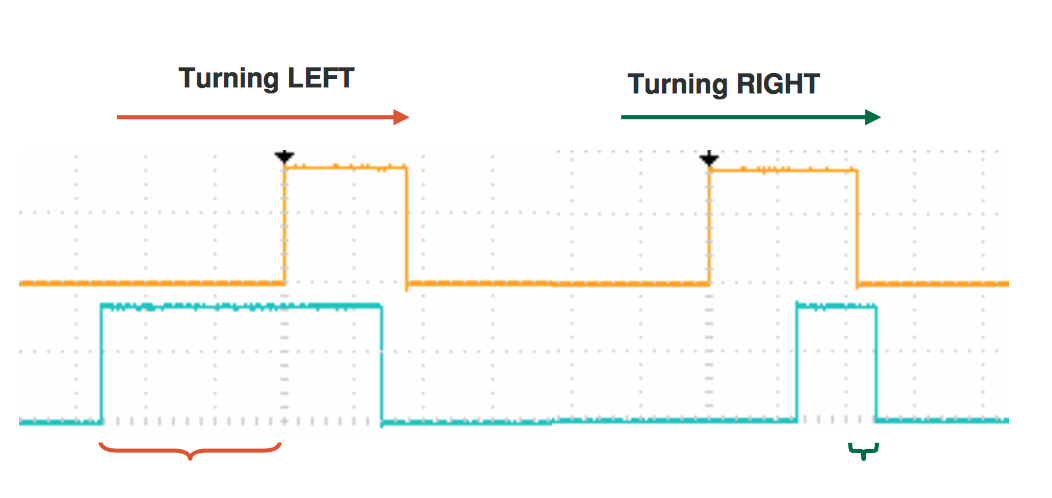
\includegraphics[width=\textwidth]{images/lab2_fig6.png}


\section{Conclusion}

\end{document}